
\chapter{Introduction}

Drone Software developments are gaining business and commercial interests.
The industry is set to become the next high growth market with very high potential and exponential growth.

\section{System Overview}


In high-level abstraction, the components of the flight stack consist of three main components ground control station, drone, and Communication Layer.
\hyperref[fig:systemoverview]{Figure 1.1} Describes the system overview. 
 \begin{figure}[H]
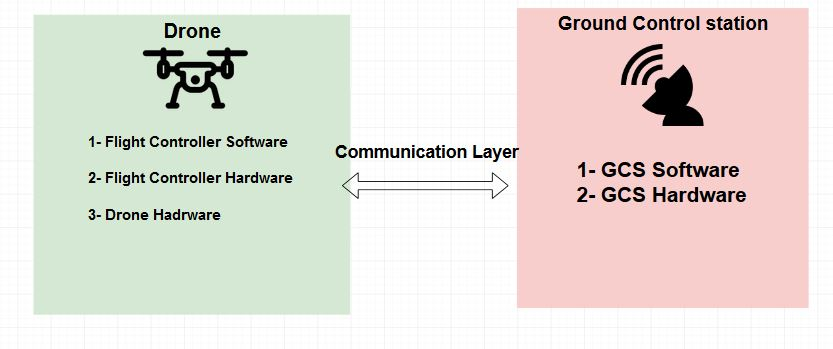
\includegraphics[width=12cm,height=10cm]{images/1.jpg}
\caption{Flight Stack Overview}
\label{fig:systemoverview}
\end{figure}
\cleardoublepage



\noindent \textbf{The Ground Control Station} is mainly an offboard computer that can communicate with the drone to gather information, for instance, location speed battery info. in addition, it's also can send a command to do certain behaviors like landing the drone or directing the drone to a specific destination.
It could also preceived as a computer with USB in a telemetry module there is also software or a user interface layer for doing specific functionality and sending commands using Mavlink communication protocol. for example Dronekit, which is a software for controlling the drone using Python. 

\textbf{Drone Hardware} consists of motors GPs probes that made up the drone.
The Flight Control Hardware is connected to Drone Hardware like Navio2 based on Rasperrypi
The flight controller software is a compiled code that uploaded to the autopilot hardware that controls the drone's basic components For example, the open source px4 and ardupilot. Additionally, the Drone hardware and the flight controller hardware could be replaced by Software in the Loop SITL it's mainly a simulation running on the computer that facilitates the whole process as a virtual instance this will practice and facilitate testing. \\ 

\textbf{Communication Layer} is a standard protocol that used for the communication between the ground control station and the drone in a bidirectional way, in another word it is like a standard collection of messages. Mavlink[1] has a standard message structure each Mavlink message has the same message structure allowing the sending node to package the information in a consistent manner and the receiving node to interpret the incoming data consistently. Every message has a message ID which a number that has an objective meaning. for example, a heartbeat is a message with id 0 when which means the drone is active.



\section{Mavlink Message Structure}


Each Mavlink message consists of 6 bytes for the header and 9 bytes for the payload and 2 bytes for the checksum for verifying the message integrity and assuring that the message wasn’t altered during the transmission. The header contains a packet start sign encoded into one byte which indicates the starting of the packet.
\begin{itemize}
  \item Each message starts with 0xFE indicates the starting of a new message.
  \item Payload length indicates the length of the following payload.
  \item Packet sequence for sequencing the packets thus it’s a method to detect packet loss.
\item System Id to identify the system ground always 1-255 similar to IP address 1 for the drone and 255 for the ground control station.
\item Component id to identify the component sending the message inside the system usually zero it’s similar to the port number but not widely used.
\item Message-id: identify the type of message in the payload for instance 0 is the heartbeat 33 it means the message is carrying out the GPs coordinates.
\item Data: payload and it depends on the message-id.
\item Last two bytes are for identifying the checksum.
\end{itemize}

\hyperref[fig:Mavlinkmessage]{Figure 1.2} Describes Mavlink message structure. 
 \begin{figure}[H]
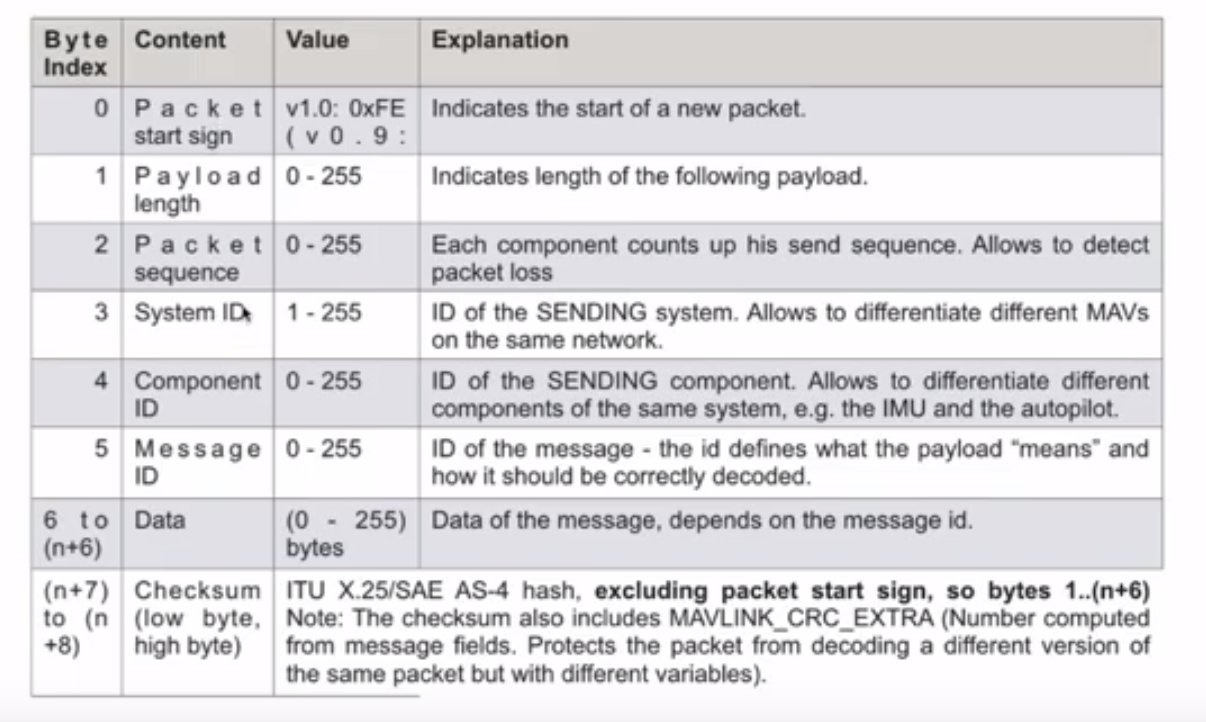
\includegraphics[width=15cm,height=10cm]{images/2.png}
\caption{Mavlink Message Structure }
\label{fig:Mavlinkmessage}
\end{figure}

\cleardoublepage



\section{Multiwii Serial Protocol MSP}

MSP MultiWii Serial Protocol[2] is the de-facto standard to interact with a MultiWii flight controller (FC). Its implementation contains a list of the most common operations one would expect from a remote control/telemetry point of view. Developers can add custom functionality if required,
They are three type of messages in MSP protocol. 
\begin{itemize}
  \item  command – is an incoming (into FC) message without implicit outgoing response from the controller
  \item  request –  is an incoming message with implicit outgoing response (e.g. a telemetry request sent in by a remote station)
  \item  response – is the outgoing message resulting from an incoming request. 
\end{itemize}

\subsection{Header}
The header is three bytes and contains the message start characters \$M and a character showing which direction the message is going. <  denotes going to the flight controller (command and request), > denotes coming from the flight controller (response).

\subsection{Size}
The fourth byte is the length (in bytes) of the data section. For example, if the data section had three INT 16 variables then the size byte would be 6.

\subsection{Type}
The 5th byte is the type of MSP message similar to Mavlink message ID. Value 1xx identify requests while 2xx identify commands.
A full list of MSP[2]

\subsection{Data}
The data is where all the information is sent. Request messages have no data in them. Commands and responses do, because they contain information.

\subsection{Checksum}
The final byte of an MSP message is the checksum. "The checksum is the XOR of size, type and payload bytes". For a request message the checksum is equal to the type.

\hyperref[fig:msp]{Figure 1.3} Depicts MSP message structure. 
 \begin{figure}[H]
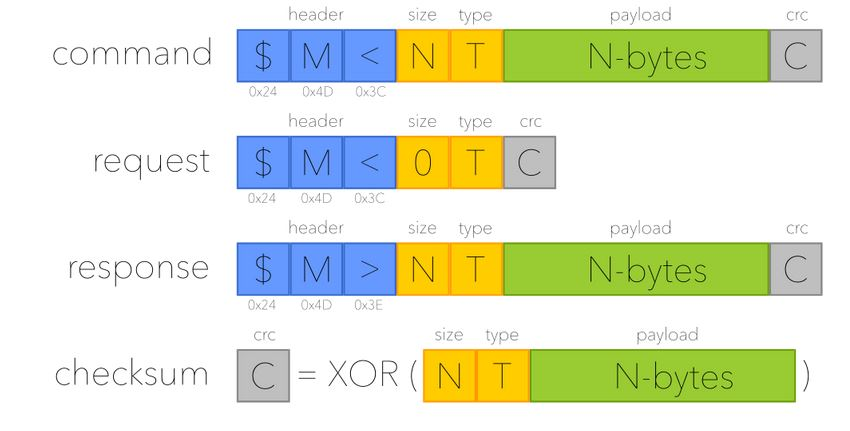
\includegraphics[width=15cm,height=10cm]{images/3.jpg}
\caption{MSP Message Structure }
\label{fig:msp}
\end{figure}



